% This file was created with tikzplotlib v0.10.1.post5.
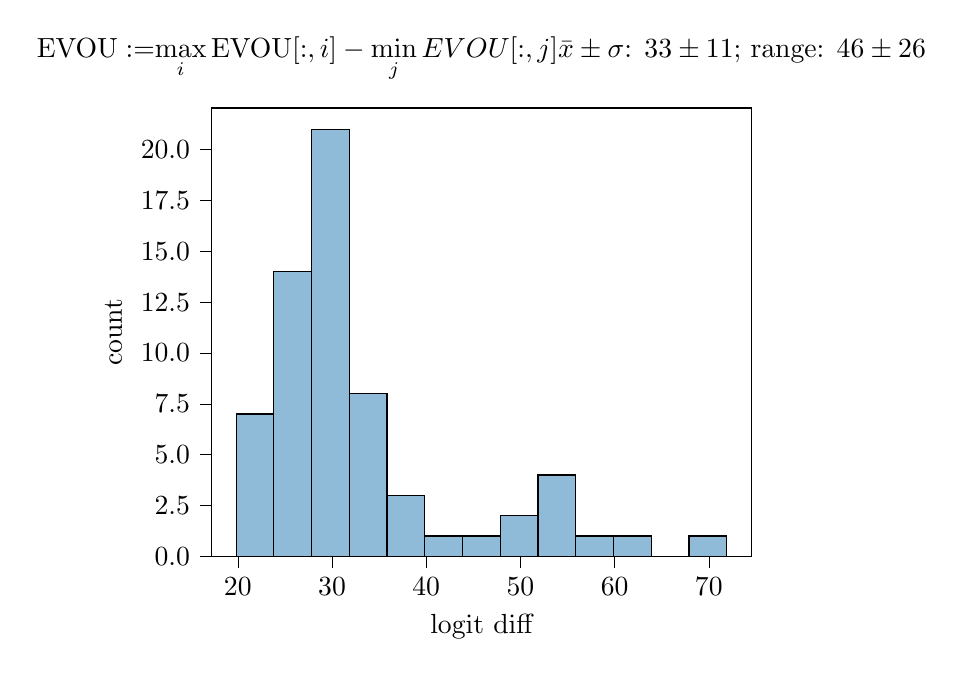
\begin{tikzpicture}

\definecolor{darkgray176}{RGB}{176,176,176}
\definecolor{steelblue31119180}{RGB}{31,119,180}

\begin{axis}[
tick align=outside,
tick pos=left,
title={\(\displaystyle \mathrm{EVOU} := \WE \WV \WO\WU \)\\
\(\displaystyle \max_i\mathrm{EVOU}[:,i] - \min_jEVOU[:,j]\)\\
\(\displaystyle \bar{x}\pm\sigma\): \(\displaystyle 33 \pm 11\); range: \(\displaystyle 46 \pm 26\)},
x grid style={darkgray176},
xlabel={logit diff},
xmin=17.2142400741577, xmax=74.4985704421997,
xtick style={color=black},
xtick={10,20,30,40,50,60,70,80},
xticklabels={
  \(\displaystyle {10}\),
  \(\displaystyle {20}\),
  \(\displaystyle {30}\),
  \(\displaystyle {40}\),
  \(\displaystyle {50}\),
  \(\displaystyle {60}\),
  \(\displaystyle {70}\),
  \(\displaystyle {80}\)
},
y grid style={darkgray176},
ylabel={count},
ymin=0, ymax=22.05,
ytick style={color=black},
ytick={0,2.5,5,7.5,10,12.5,15,17.5,20,22.5},
yticklabels={
  \(\displaystyle {0.0}\),
  \(\displaystyle {2.5}\),
  \(\displaystyle {5.0}\),
  \(\displaystyle {7.5}\),
  \(\displaystyle {10.0}\),
  \(\displaystyle {12.5}\),
  \(\displaystyle {15.0}\),
  \(\displaystyle {17.5}\),
  \(\displaystyle {20.0}\),
  \(\displaystyle {22.5}\)
}
]
\draw[draw=black,fill=steelblue31119180,fill opacity=0.5] (axis cs:19.8180732727051,0) rectangle (axis cs:23.8239705012395,7);
\draw[draw=black,fill=steelblue31119180,fill opacity=0.5] (axis cs:23.8239705012395,0) rectangle (axis cs:27.8298677297739,14);
\draw[draw=black,fill=steelblue31119180,fill opacity=0.5] (axis cs:27.8298677297739,0) rectangle (axis cs:31.8357649583083,21);
\draw[draw=black,fill=steelblue31119180,fill opacity=0.5] (axis cs:31.8357649583083,0) rectangle (axis cs:35.8416621868427,8);
\draw[draw=black,fill=steelblue31119180,fill opacity=0.5] (axis cs:35.8416621868427,0) rectangle (axis cs:39.8475594153771,3);
\draw[draw=black,fill=steelblue31119180,fill opacity=0.5] (axis cs:39.8475594153771,0) rectangle (axis cs:43.8534566439115,1);
\draw[draw=black,fill=steelblue31119180,fill opacity=0.5] (axis cs:43.8534566439115,0) rectangle (axis cs:47.8593538724459,1);
\draw[draw=black,fill=steelblue31119180,fill opacity=0.5] (axis cs:47.8593538724459,0) rectangle (axis cs:51.8652511009803,2);
\draw[draw=black,fill=steelblue31119180,fill opacity=0.5] (axis cs:51.8652511009803,0) rectangle (axis cs:55.8711483295147,4);
\draw[draw=black,fill=steelblue31119180,fill opacity=0.5] (axis cs:55.8711483295147,0) rectangle (axis cs:59.8770455580491,1);
\draw[draw=black,fill=steelblue31119180,fill opacity=0.5] (axis cs:59.8770455580491,0) rectangle (axis cs:63.8829427865835,1);
\draw[draw=black,fill=steelblue31119180,fill opacity=0.5] (axis cs:63.8829427865835,0) rectangle (axis cs:67.8888400151179,0);
\draw[draw=black,fill=steelblue31119180,fill opacity=0.5] (axis cs:67.8888400151179,0) rectangle (axis cs:71.8947372436523,1);
\end{axis}

\end{tikzpicture}
